\chapter{Research Methodology}

The important aspect of the approach is that we are analyzing the programs statically. This helps us check each and every possible case that may occur during execution of the programs. To implement the current idea of detecting critical sections, we have designed architecture as follows.


\begin{figure}[H]
\centering
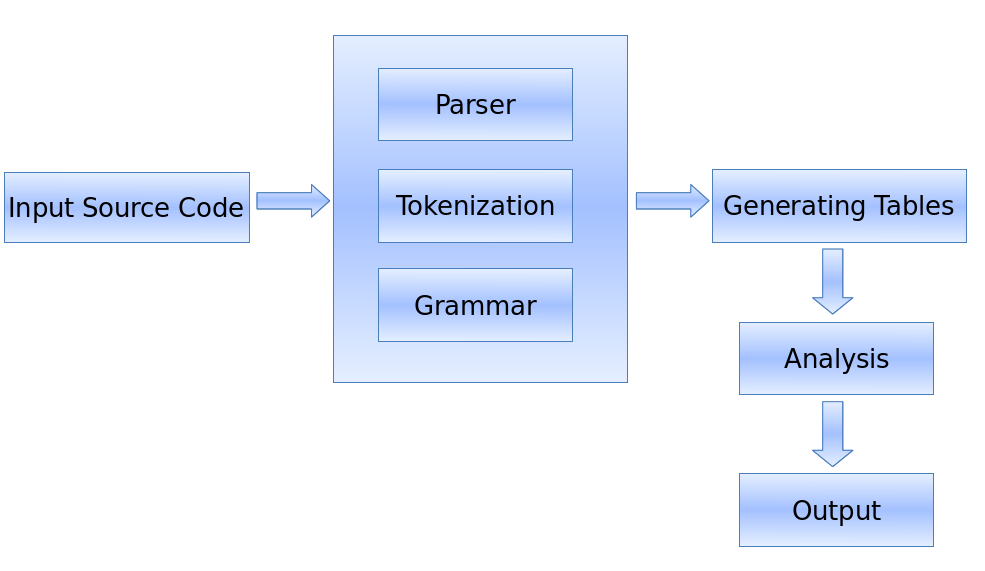
\includegraphics[scale=0.4]{architecture.png}
\caption{Architectural Diagram}
\label{<<Label>>}
\end{figure}

\section{Architecture}

\subsection{Input Source Files}
A normal multithreaded program is given as input with critical sections. This file is first compiled to check for errors and only when it is compiled error free; it heads to the next stage.
\begin{figure}[H]
\centering
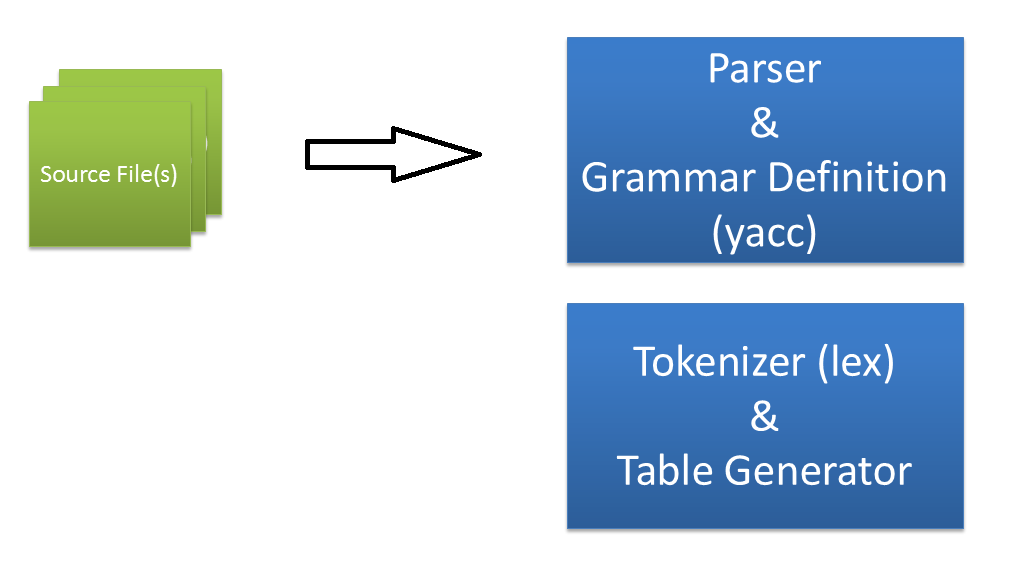
\includegraphics[scale=0.4]{input.png}
\caption{Input}
\label{<<Label>>}
\end{figure}

\subsection{Parser, Tokenizer, Grammar}
Flex (The Fast Lexical Analyser) is a tool for generating scanners. A scanner, sometimes called a tokenizer, is a program which recognizes lexical patterns in text. The flex program reads user-specified input files, or its standard input if no file names are given, for a description of a scanner to generate [4].

With it we separate all the unwanted text (ex. Comments, pre-processors) and tokenize the program to find out shared memory, functions, threads, and locks. In order to find the above from the token, it analyzes its input for occurrences of text matching the regular expressions for each rule. Whenever it finds a match, it executes the corresponding code [3].

The different in-built functions were monitoring are:\\
\begin{itemize}
\item pthread\_create
\item pthread\_join
\item pthread\_cond\_wait
\item pthread\_cond\_signal
\item sem\_wait
\item sem\_post
\end{itemize}
\begin{figure}[H]
\centering
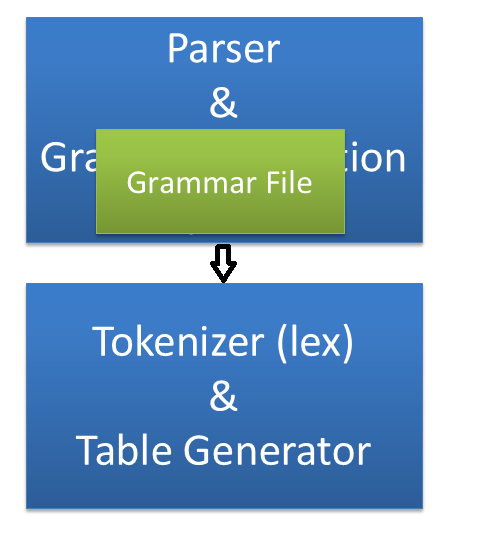
\includegraphics[scale=0.4]{grammar.png}
\caption{Parsing}
\label{<<Label>>}
\end{figure}


\subsection{Generating Tables}
Yacc (Yet Another Compiler Compiler) provides a general tool for describing the input to a computer program. We specify the structures of the input, together with code to be invoked as each such structure is recognized. Yacc turns such a specification into a subroutine that handles the input process; frequently, it is convenient and appropriate to have most of the flow of control in the user's application handled by this subroutine.

The input subroutine produced by Yacc calls a usersupplied routine to return the next basic input item. Thus, the user can specify his input in terms of individual input characters or in terms of higher level constructs such as names and numbers. The user-supplied routine may also handle idiomatic features such as comment and continuation conventions, which typically defy easy grammatical specification [5]. 

Once all the unwanted text is ignored from the code, with the help of Yacc we generate the following data structures:

\begin{itemize}
\item Global variables’ table (Id, access, variable\_name, line\_number)\\
Stores the entries of all the shared variables that exist in the program

\item User-defined Functions (Id, function\_name, return\_type, number\_of\_parameters, line\_number)\\
Stores the entries of all the functions defined by the user in the program.

\item Functions’ Local symbol table (Id, access\_type, name, data\_type, function\_id, line\_number)\\
Stores all the local variables associated with a function.

\item Semaphore table (id, name, function, location)\\
Stores all the locations of sem\_wait() and sem\_post functions used in the code

\item Thread table (Id, thread\_name, function\_name, function\_id, thread\_attribute, parameters, parent\_thread)\\
Stores all the threads associated with which functions and their attributes

\item Shared Memory Log table (Id, function\_name, shared\_object, scope, line\_number, thread-function\_id, thread\_id)\\
Stores a log of all variables which may cause data races and helps analysis the proof.

\item Critical Section table (Id, shared\_object, thread\_function\_index, first\_location, last\_location, function\_name)

\end{itemize}
\begin{figure}[H]
\centering
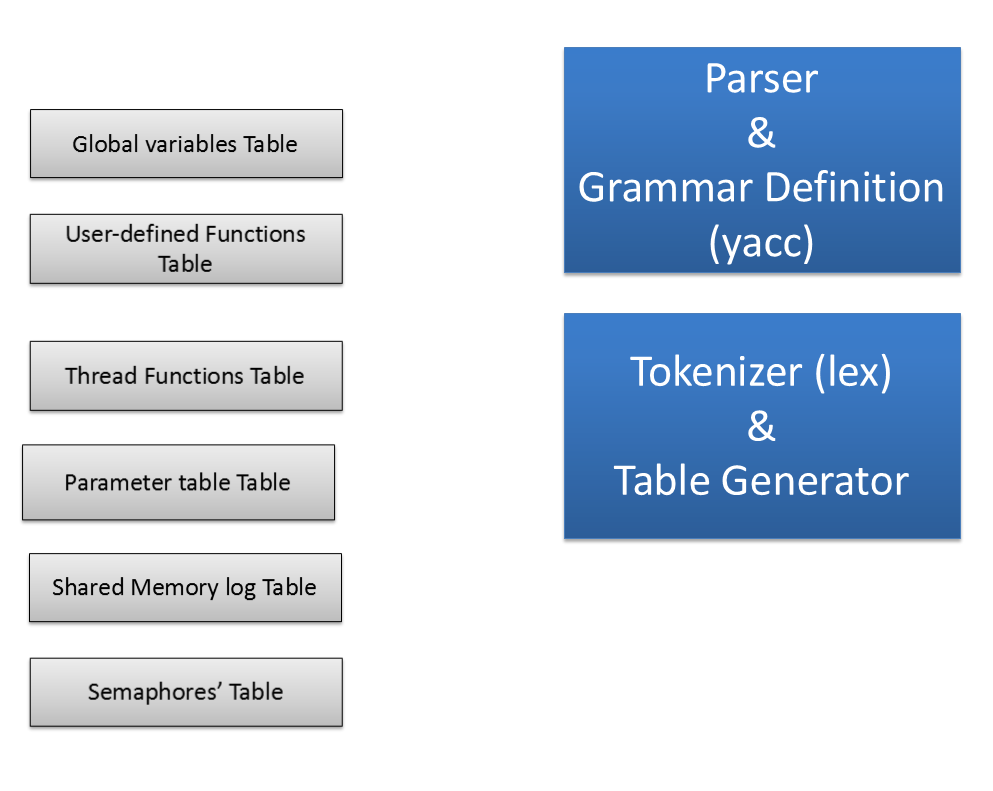
\includegraphics[scale=0.5]{tables.png}
\caption{Tables}
\label{<<Label>>}
\end{figure}

\subsection{Analysis}
Once all tables are generated we analyze them. If any shared variable exists in multiple functions and is unhandled i.e. it is not protected with the function calls sem\_wait(), sem\_post(), then we categorize that shared variable as unhandled critical section and add its entry to the critical section table.

After getting a table having all the unhandled critical sections, we analyze it for the location where we need to provides locks and unlocks. 

From the Critical Section Table, we get the line numbers of first and last occurrence of shared variables’ usage. Depending on their closeness, we decide the number of times we need to lock, and unlock.

\subsection{Output}
Once all tables are analyzed and we display all the unhandled critical sections that exist. The various attributes of the critical sections that are found are: 
\begin{itemize}

\item The shared object which is being accessed my multiple threads

\item The threads which are accessing the same shared object

\item The functions in which the critical section exist

\item The location pertaining to the line number of the critical section

\end{itemize}

\begin{figure}[H]
\centering
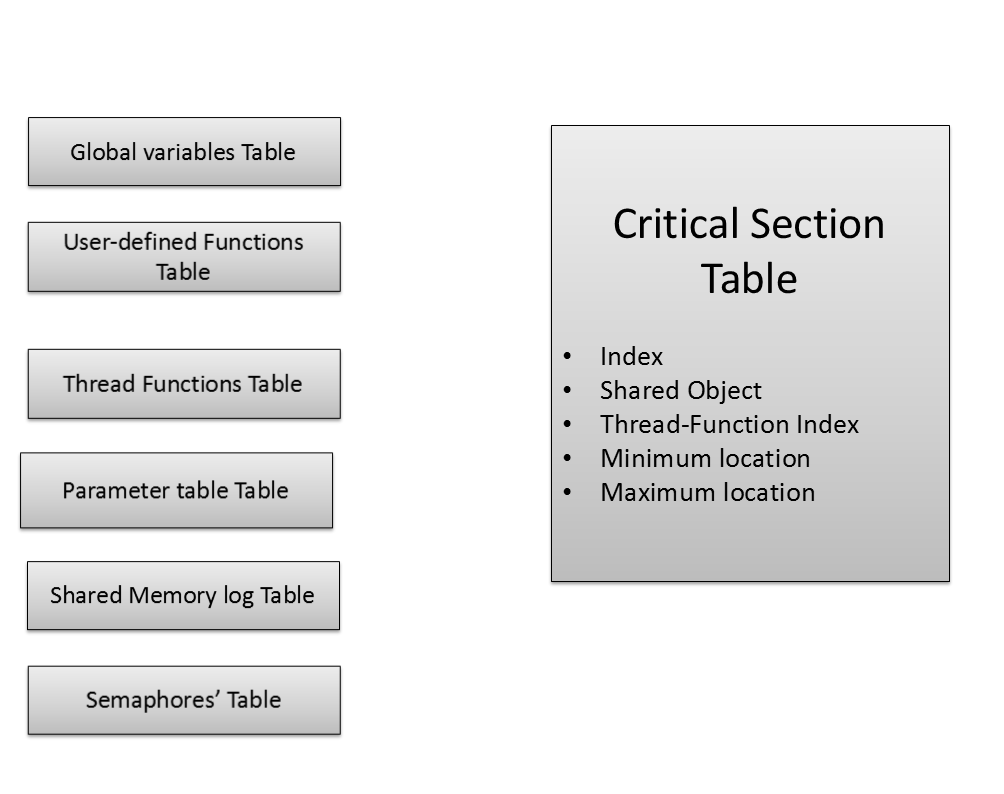
\includegraphics[scale=0.5]{cs.png}
\caption{Contents of Critical Section Table}
\label{<<Label>>}
\end{figure}

We then decide if the programmer handles the critical sections himself, or we have to handle it. Once the permissions are given, we add sem\_wait() sem\_post(), recompile the code to produce bug free programs.

\section{Placement of our tool in GCC hierarchy}
Our tool exists adjacent to the current architecture of GCC but runs once the compilation is over and no errors are generated. It keeps a copy of the original source code, works on it, and pushes its warnings along with the warnings of the compiler.
\begin{figure}[H]
\centering
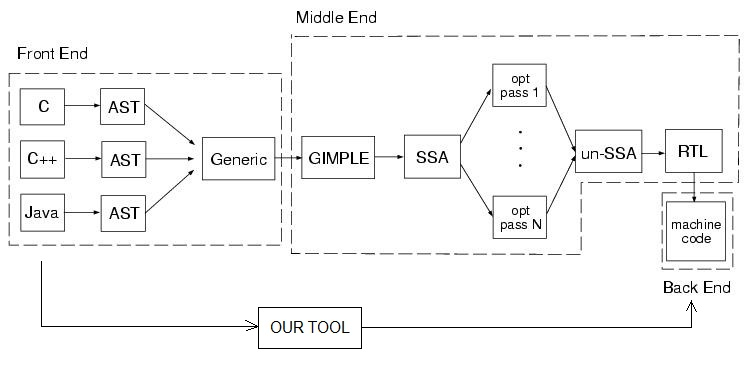
\includegraphics[scale=0.6]{gcc.jpg}
\caption{Integration of our tool in GCC}
\label{<<Label>>}
\end{figure}


